\clearpage\section{Resultados y análisis}

\subsection{Experimento 5: escalabilidad espacial}

\begin{table}[H]\centering\small
\caption{k-NN y radio planar de 0.02 grados; doce centros por tamaño.}
\begin{tabular}{@{}lrrrrr@{}}\toprule
N & Consulta & Método & Lecturas & Media ms & Desv. ms \\ \midrule
10000 & k=20 & Sequential & 60.00 & 9.74 & 1.95 \\
10000 & k=20 & RTree & 10.67 & 1.85 & 0.43 \\
10000 & r=0.02 & Sequential & 60.00 & 9.02 & 1.40 \\
10000 & r=0.02 & RTree & 97.17 & 4.00 & 1.16 \\
50000 & k=20 & Sequential & 296.00 & 40.20 & 2.34 \\
50000 & k=20 & RTree & 16.92 & 2.68 & 0.60 \\
50000 & r=0.02 & Sequential & 296.00 & 37.89 & 3.48 \\
50000 & r=0.02 & RTree & 631.92 & 12.85 & 1.48 \\
100000 & k=20 & Sequential & 590.00 & 108.20 & 9.69 \\
100000 & k=20 & RTree & 25.17 & 4.93 & 1.26 \\
100000 & r=0.02 & Sequential & 590.00 & 95.14 & 9.69 \\
100000 & r=0.02 & RTree & 1381.42 & 35.71 & 5.47 \\
\bottomrule\end{tabular}\end{table}

\begin{figure}[H]\centering
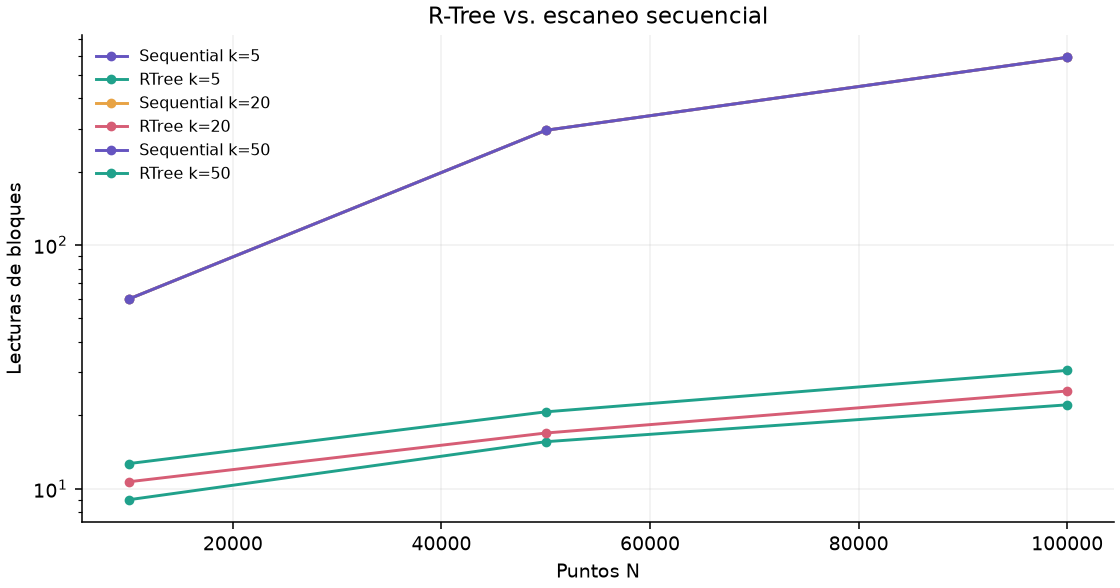
\includegraphics[width=.89\textwidth]{../benchmarks/p2/results/exp5_spatial.png}
\caption{Escalabilidad k-NN para k=5,20,50. Eje de I/O logarítmico.}\end{figure}

Con 100000 puntos y k=20, el R-Tree leyó 25.17 bloques en promedio frente a 590.00 del escaneo. La poda evita recorrer la mayoría de las páginas en este conjunto 2D. La comparación k-NN devuelve identificadores: no incluye recuperar filas comerciales del Heap. En radios sí se contabiliza el refinamiento desde el archivo de puntos. Los CSV crudos incluyen los tres radios y todos los k.

En radio r=0.02 y N=100000, el R-Tree con refinamiento lee 1381.42 bloques, más que el escaneo. Los candidatos espaciales están dispersos en el archivo y provocan relecturas con la caché acotada. Aun así, su latencia es menor al evaluar menos puntos. Un índice selectivo no garantiza por sí solo menor I/O al recuperar datos no agrupados.

\clearpage\subsection{Experimento 5: efecto de la dimensión}

\begin{table}[H]\centering\small
\caption{2000 vectores uniformes por dimensión, doce consultas k=10.}
\begin{tabular}{@{}lrrrr@{}}\toprule
D & Scan I/O & R-Tree I/O & Scan ms & R-Tree ms \\ \midrule
2 & 13.00 & 6.50 & 3.69 & 2.13 \\
4 & 21.00 & 8.83 & 3.09 & 2.77 \\
8 & 37.00 & 41.58 & 4.28 & 9.64 \\
16 & 68.00 & 98.00 & 5.66 & 23.31 \\
32 & 135.00 & 174.00 & 9.51 & 45.16 \\
64 & 287.00 & 385.00 & 16.41 & 96.50 \\
128 & 668.00 & 1104.00 & 30.34 & 238.83 \\
\bottomrule\end{tabular}\end{table}

\begin{figure}[H]\centering
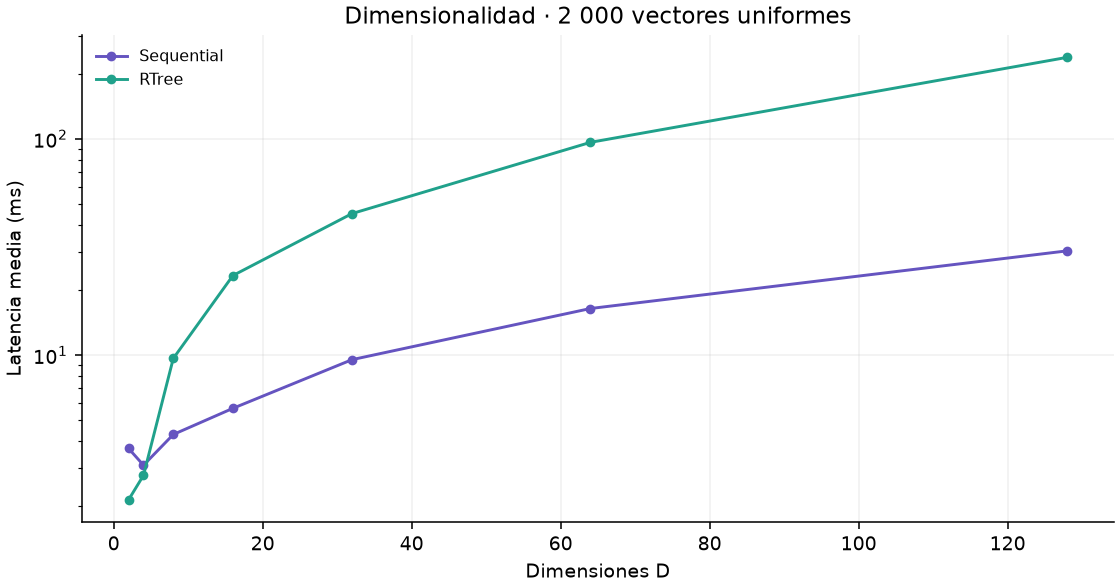
\includegraphics[width=.89\textwidth]{../benchmarks/p2/results/exp5_dimensions.png}
\caption{Costo temporal al aumentar D; escala logarítmica.}\end{figure}

El primer D medido donde la media del árbol supera al escaneo es 8. A dimensiones elevadas, la búsqueda visita una fracción creciente del árbol y disminuye el fan-out. Este cruce depende de la distribución, la implementación y el hardware; no debe generalizarse como una dimensión límite universal.

\clearpage\subsection{Experimento 6: construcción y espacio}

\begin{table}[H]\centering\small
\caption{Construcción y tamaño del diccionario/posteos propios frente al índice GIN.}
\begin{tabular}{@{}lrrr@{}}\toprule
N & Método & Construcción ms & Índice KiB \\ \midrule
1000 & Inverted & 194.62 & 304.0 \\
1000 & PostgreSQL GIN & 228.02 & 104.0 \\
5000 & Inverted & 853.07 & 1072.0 \\
5000 & PostgreSQL GIN & 123.42 & 304.0 \\
10000 & Inverted & 1699.46 & 1964.0 \\
10000 & PostgreSQL GIN & 156.66 & 536.0 \\
20000 & Inverted & 3340.37 & 3624.0 \\
20000 & PostgreSQL GIN & 273.10 & 960.0 \\
\bottomrule\end{tabular}\end{table}

\begin{figure}[H]\centering
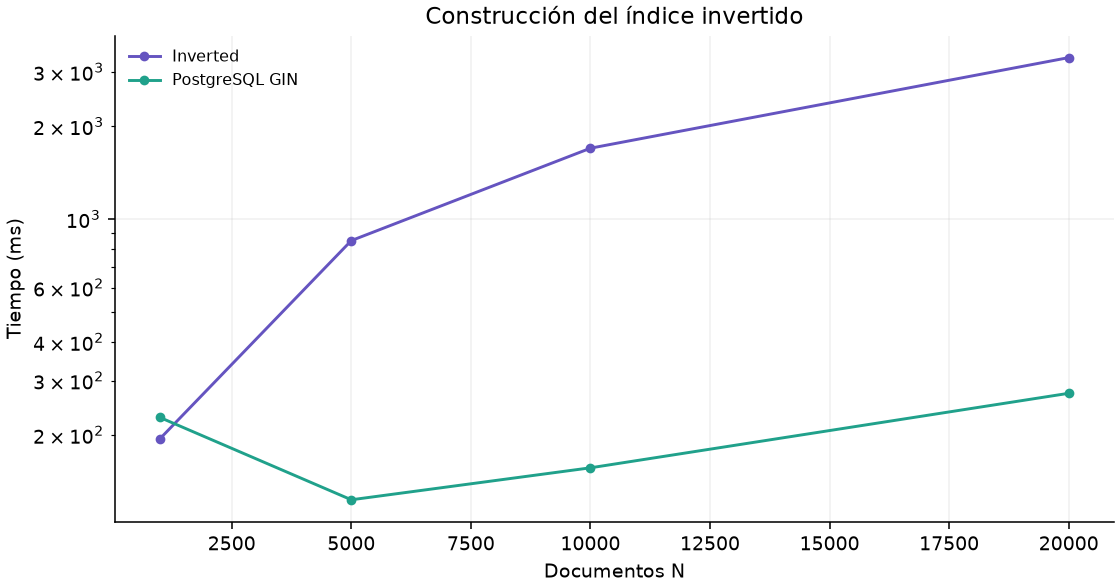
\includegraphics[width=.48\textwidth]{../benchmarks/p2/results/exp6_build.png}
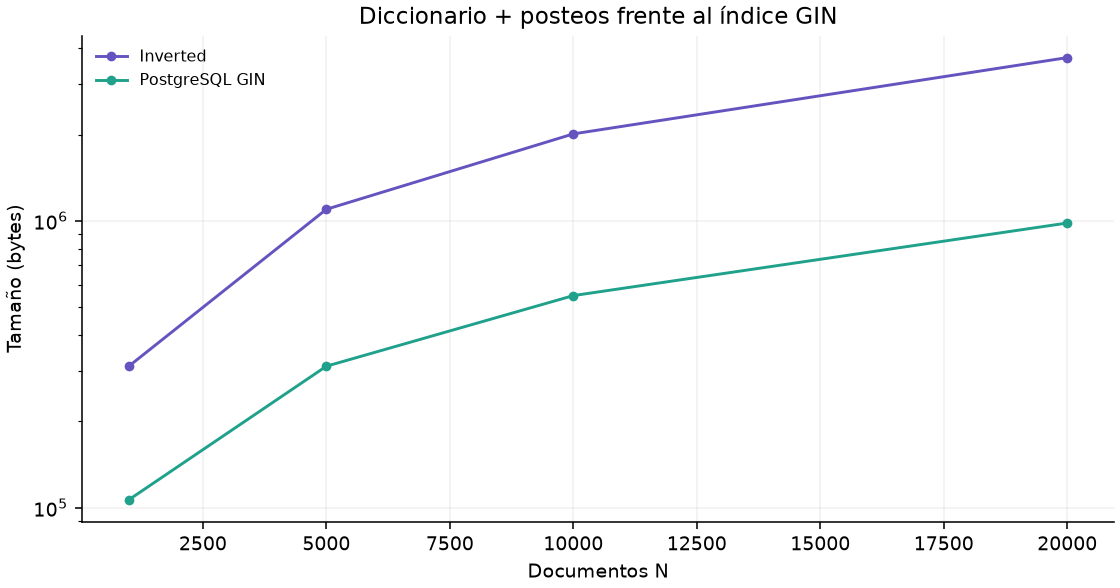
\includegraphics[width=.48\textwidth]{../benchmarks/p2/results/exp6_size.png}
\caption{Crecimiento temporal y espacial. Los archivos de normas se excluyen del tamaño propio solicitado.}\end{figure}

El índice propio usa registros de diccionario de tamaño fijo y posteos sin compresión; GIN utiliza una representación distinta y comprime identificadores. Los costos de construcción también incluyen trabajo diferente de normalización y de base de datos, por lo que la tabla describe implementaciones completas bajo las condiciones documentadas, no una comparación aislada de un algoritmo idéntico.

\clearpage\subsection{Experimento 6: consultas y transferencias}

\begin{table}[H]\centering\footnotesize\renewcommand{\arraystretch}{1.0}
\caption{Latencias medias sobre 20000 documentos; tres consultas distintas por combinación.}
\begin{tabular}{@{}lrrrr@{}}\toprule
Términos & Consulta & Full Scan ms & Invertido ms & GIN ms \\ \midrule
1 & AND & 325.70 & 4.94 & 2.91 \\
1 & OR & 321.58 & 5.36 & 2.74 \\
1 & AND-NOT & 325.85 & 5.09 & 2.76 \\
1 & RANK & 349.69 & 35.44 & 56.66 \\
3 & AND & 321.56 & 18.98 & 2.15 \\
3 & OR & 325.34 & 21.08 & 6.37 \\
3 & AND-NOT & 320.30 & 20.98 & 2.61 \\
3 & RANK & 369.49 & 134.17 & 601.88 \\
5 & AND & 322.86 & 21.09 & 1.49 \\
5 & OR & 330.72 & 29.05 & 6.99 \\
5 & AND-NOT & 316.44 & 28.49 & 2.71 \\
5 & RANK & 372.73 & 146.09 & 1068.13 \\
\bottomrule\end{tabular}\end{table}

\begin{table}[H]\centering\footnotesize\renewcommand{\arraystretch}{1.0}
\caption{Transferencias Atlas y buffers PostgreSQL reportados por separado.}
\begin{tabular}{@{}lrrrrr@{}}\toprule
Términos & Consulta & Scan 4K & Inv. 4K & PG hit 8K & PG read 8K \\ \midrule
1 & AND & 6668.0 & 23.0 & 784.0 & 0.0 \\
1 & OR & 6668.0 & 23.0 & 784.0 & 0.0 \\
1 & AND-NOT & 6668.0 & 23.0 & 784.0 & 0.0 \\
1 & RANK & 6668.0 & 102.0 & 784.0 & 0.0 \\
3 & AND & 6668.0 & 84.0 & 392.0 & 0.0 \\
3 & OR & 6668.0 & 84.0 & 802.0 & 0.0 \\
3 & AND-NOT & 6668.0 & 84.0 & 550.3 & 0.0 \\
3 & RANK & 6668.0 & 319.0 & 802.0 & 0.0 \\
5 & AND & 6668.0 & 103.7 & 19.3 & 0.0 \\
5 & OR & 6668.0 & 103.7 & 806.7 & 0.0 \\
5 & AND-NOT & 6668.0 & 103.7 & 540.7 & 0.0 \\
5 & RANK & 6668.0 & 471.0 & 806.7 & 0.0 \\
\bottomrule\end{tabular}\end{table}

OR y ranking consultan conjuntos mayores cuando los términos son frecuentes. AND puede reducir resultados por intersección. Los planes PostgreSQL completos permiten distinguir navegación GIN, acceso a Heap y ordenamiento. El ranking ts\_rank\_cd tiene costo y semántica diferentes de TF-IDF/coseno; una menor latencia de Atlas en un caso no demuestra superioridad general frente a PostgreSQL.

\begin{figure}[H]\centering
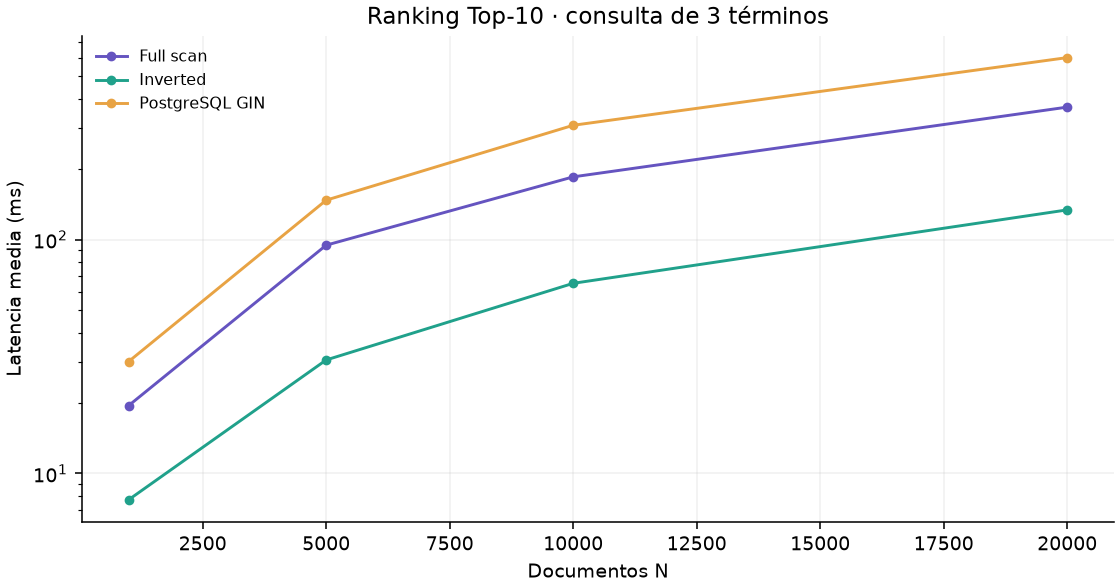
\includegraphics[width=.66\textwidth]{../benchmarks/p2/results/exp6_query.png}
\caption{Ranking Top-10 de tres términos según tamaño del corpus.}\end{figure}

\clearpage\subsection{Experimento 7: BoVW frente a embeddings}

\begin{table}[H]\centering\small
\caption{100 imágenes de consulta excluidas del corpus indexado.}
\begin{tabular}{@{}lrrrr@{}}\toprule
Método & P@5 & P@10 & Consulta ms & Extracción ms/img \\ \midrule
BoVW & 0.330 & 0.295 & 164.35 & 7.07 \\
ResNet18+IVF & 0.702 & 0.688 & 35.00 & 26.16 \\
\bottomrule\end{tabular}\end{table}

\begin{figure}[H]\centering
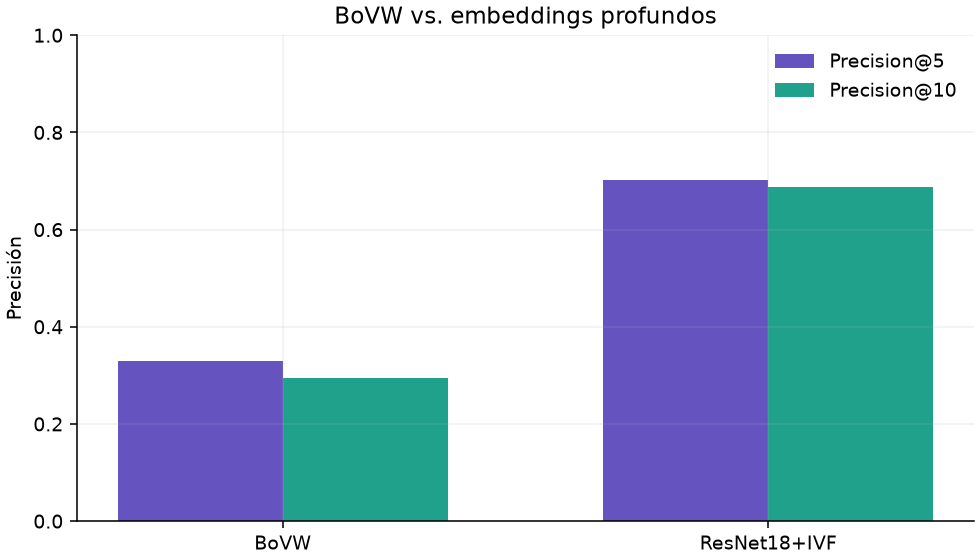
\includegraphics[width=.89\textwidth]{../benchmarks/p2/results/exp7_quality.png}
\caption{Relevancia definida por igualdad de articleType.}\end{figure}

ResNet-18 obtuvo mayor precisión por categoría en este conjunto. BoVW reconoce patrones locales que pueden repetirse entre objetos de categorías distintas, mientras las características profundas incorporan representaciones aprendidas en ImageNet. La extracción densa es más costosa por imagen en la CPU usada. La consulta BoVW incluye cuantización contra el codebook; su carga inicial se reutiliza en este benchmark. Los tiempos de extracción son medias de lotes de preparación, no latencias individuales de una imagen interactiva.

\clearpage\subsection{Experimento 8: recall, latencia e I/O}

\begin{table}[H]\centering\small
\caption{Compromiso de IVF contra la búsqueda exacta sobre las mismas 100 consultas.}
\begin{tabular}{@{}lrrrr@{}}\toprule
Probes & Recall@10 & Media ms & Desv. ms & Lecturas medias \\ \midrule
1 & 67.2\% & 13.05 & 4.10 & 228.63 \\
2 & 86.2\% & 18.64 & 6.08 & 351.33 \\
5 & 97.1\% & 34.09 & 11.39 & 690.03 \\
10 & 99.2\% & 60.63 & 18.65 & 1251.39 \\
20 & 99.8\% & 112.63 & 32.20 & 2331.02 \\
50 & 100.0\% & 239.19 & 50.95 & 4962.69 \\
100 & 100.0\% & 477.61 & 75.26 & 10103.00 \\
\bottomrule\end{tabular}\end{table}

\begin{figure}[H]\centering
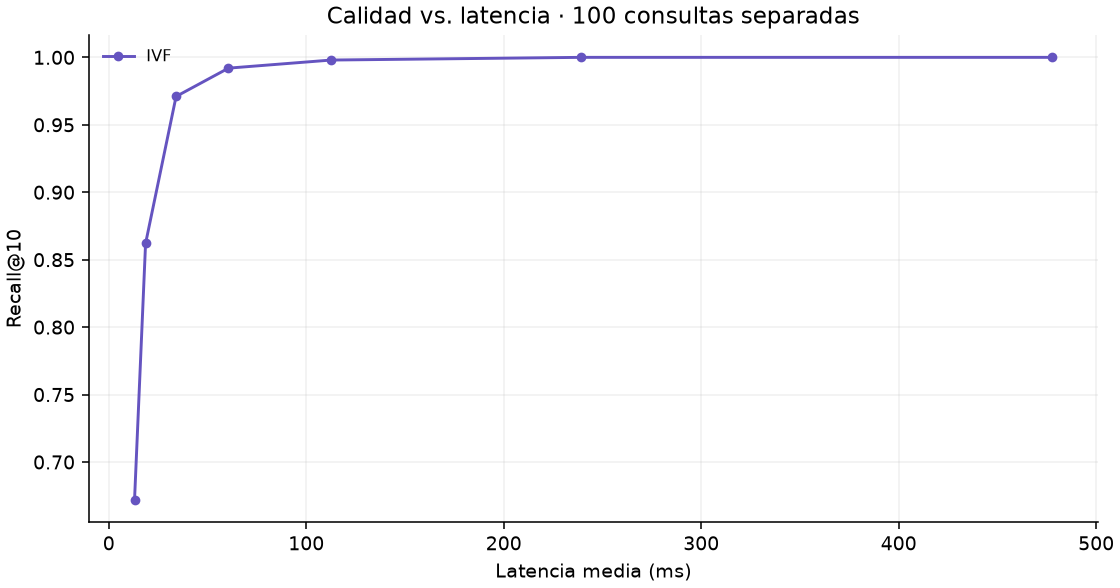
\includegraphics[width=.48\textwidth]{../benchmarks/p2/results/exp8_recall_latency.png}
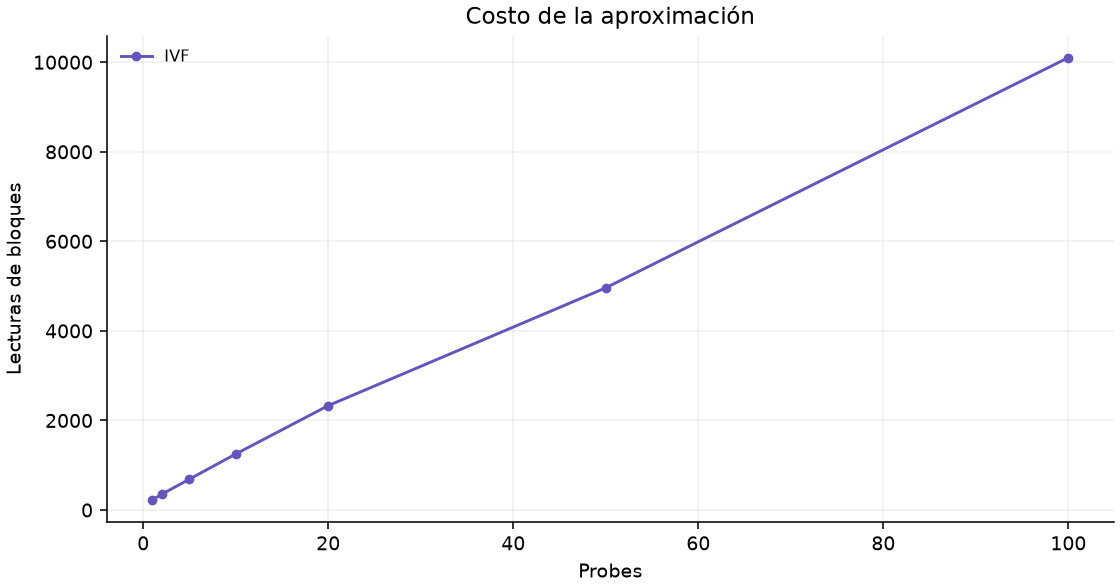
\includegraphics[width=.48\textwidth]{../benchmarks/p2/results/exp8_reads.png}
\caption{La exploración de más listas aumenta calidad y costo de consulta.}\end{figure}

Cinco probes ofrecen un punto de operación favorable en estas mediciones: 97.1\% de recall medio, sin explorar todo el índice. Los cien probes recorren todas las listas y garantizan la equivalencia con el escaneo exacto. Un recall de 100\% observado con menos probes solo aplica a las consultas medidas. La latencia incluye directorio y apertura; el conteo incluye metadata y listas, no recuperación de la ficha comercial.
